\documentclass[a4j]{jreport}
\usepackage{alltt}
\usepackage{ascmac}
\usepackage{color}
\usepackage{dirtree}
\usepackage{float}
\usepackage[dvipdfmx]{graphicx}
\usepackage{url}

\begin{document}

\title{Linuxの教科書}
\author{須栗歩人}
\maketitle

% 目次
\tableofcontents

% 章
\chapter{おぼえておきたいコマンド}

Linuxのデスクトップ環境では、Linuxコマンドを知らなくともGUI操作で多くのことができます。しかしそれでも、いくつかのコマンドを知っていればさらに便利で、かつ、LinuxというOSを理解するのに役立ちます。

\begin{figure}[H]
	\centering
	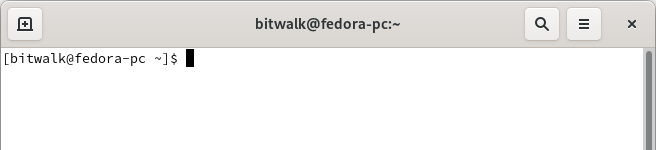
\includegraphics[width=10cm]{pic/gnome-terminal.png}
	\caption{ターミナルエミュレーター}
\end{figure}

Linuxを使うために、とりあえずおぼえておきたいコマンドをまとめました。\\

%%% ls
\section{\texttt{ls} --- ファイルやディレクトリの参照}

【ファイルとファイルシステム管理】\\

\texttt{ls}は、ファイルの一覧を表示するコマンドです。\\

\begin{itembox}[l]{使用例}
	\begin{alltt}\texttt{\$ ls
		ダウンロード  デスクトップ  ビデオ  画像
		テンプレート  ドキュメント  音楽    公開}\end{alltt}
\end{itembox}

%%% cp
\section{\texttt{cp} --- ファイルのコピー}

【ファイルとファイルシステム管理】\\

\texttt{cp}は、ファイルをある場所から別の場所へコピーするコマンドです。\\

\begin{itembox}[l]{使用例}
	\begin{alltt}\texttt{\$ cp \textit{filename1 filename2}}\end{alltt}
\end{itembox}

%%% mv
\section{\texttt{mv} --- ファイルの移動}

【ファイルとファイルシステム管理】\\

\texttt{mv}は、ファイルやディレクトリの移動、名前の変更をするコマンドです。\\

\begin{itembox}[l]{使用例}
	\begin{alltt}\texttt{\$ mv \textit{filename1 filename2}}\end{alltt}
\end{itembox}

%%% rm
\section{\texttt{rm} --- ファイルの削除}

【ファイルとファイルシステム管理】\\

\texttt{rm}は、ファイルシステムよりファイルを削除するコマンドです。\\

\begin{itembox}[l]{使用例}
	\begin{alltt}\texttt{\$ rm \textit{filename}}\end{alltt}
\end{itembox}

%%% pwd
\section{\texttt{pwd} --- 現在の作業ディレクトリ名の表示}

【ファイルとファイルシステム管理】\\

\texttt{pwd}は、現在の作業ディレクトリのフルパスを出力するコマンドです。\\

\begin{itembox}[l]{使用例}
	\begin{alltt}\texttt{\$ pwd
			/home/bitwalk}\end{alltt}
\end{itembox}

%%% cd
\section{\texttt{cd} --- ディレクトリの変更}

【ファイルとファイルシステム管理】\\

\texttt{cd}は、シェル等の現在の作業ディレクトリを変更するコマンドです。\\

\begin{itembox}[l]{使用例}
	\begin{alltt}\texttt{\$ cd ダウンロード}\end{alltt}
\end{itembox}

%%% mkdir
\section{\texttt{mkdir} --- ディレクトリの作成}

【ファイルとファイルシステム管理】\\

\texttt{mkdir}は、ディレクトリを作成するコマンドです。\\

\begin{itembox}[l]{使用例}
	\begin{alltt}\texttt{\$ mkdir \textit{dirname}}\end{alltt}
\end{itembox}

%%% cat
\section{\texttt{cat} --- ファイルの内容を表示}

【ファイルとファイルシステム管理】\\

\texttt{cat}は、ファイルを連結させたり表示したりするのに用いるコマンドです。\\

\begin{itembox}[l]{使用例}
	\begin{alltt}\texttt{\$ cat .bash_profile
			# .bash_profile
			
			# Get the aliases and functions
			if [ -f ~/.bashrc ]; then
			. ~/.bashrc
			fi
			
			# User specific environment and startup programs
			\$ 
		}\end{alltt}
\end{itembox}

%%% find
\section{\texttt{find} --- ファイルの検索}

【検索】\\

\texttt{find}は、ファイルシステムの1つ以上のディレクトリツリー上で検索を行い、ユーザーが指定した基準にマッチするファイルを探すコマンドです。\\

\begin{itembox}[l]{使用例}
	\begin{alltt}\texttt{\$ }\end{alltt}
\end{itembox}

%%% which
\section{\texttt{which} --- コマンドのパスを表示}

【検索】\\

\texttt{witch}は、指定したコマンドプログラムのフルパスを検索して表示するコマンドです。\\

\begin{itembox}[l]{使用例}
	\begin{alltt}\texttt{\$ which cp
			/usr/bin/cp}\end{alltt}
\end{itembox}

%%% which
\section{\texttt{man} --- コマンドのマニュアルを表示}

【マニュアル】\\

\texttt{man}は、指定したコマンドプログラムのマニュアルを表示するコマンドです。\\

\begin{itembox}[l]{使用例}
	\begin{alltt}\texttt{\$ man ls
	LS(1)                          ユーザーコマンド                          LS(1)
	
	名前
	ls - ディレクトリの内容をリスト表示する
	
	書式
	ls [オプション]... [ファイル]...
	
	説明
	FILE   (デフォルトは現在のディレクトリ)  に関する情報を一覧表示します。
	-cftuvSUX のいずれも指定されず、 --sort も指定されていない場合、 要素は
	アルファベット順でソートされます。
	
	長いオプションで必須となっている引数は短いオプションでも必須です。
	
	-a, --all
	. で始まる要素を無視しない
	
	-A, --almost-all
	. および .. を一覧表示しない
	
	--author                -l と合わせて使用した時、各ファイルの作成者を表
	示する
	Manual page ls(1) line 1 (press h for help or q to quit)
}\end{alltt}
\end{itembox}

% 章
\chapter{ファイルシステム}

LinuxなどのUNIX系OSの標準的なディレクトリ構成を定めたFHS, \textit{Filesystem Hierarchy Standard}で、ディレクトリの名前や構成、ファイルの名前などを定めています。

多くのLinuxディストリビューションはFHS準拠しています。

\section{FHS 3.0 (2015-05-18)}
	\dirtree{%
	.1 / ファイルシステム階層全体の第一階層(ルートディレクトリ).
	.2 /bin 一般ユーザー向けの基本コマンドの実行ファイル.
	.2 /boot ブートローダー関連のファイル群.
	.2 /dev 基本デバイス.
	.2 /etc システム全体に関わる固有設定ファイル群.
	.2 /home ユーザーの ホームディレクトリ.
	.3 bitwalk(ユーザーアカウント例).
	.2 /lib 実行ファイルの基本となるライブラリ群.
	.2 /media リムーバブル媒体のマウントポイント.
	.2 /mnt ファイルシステムの一時マウントポイント.
	.2 /opt オプションパッケージのインストール用.
	.2 /proc カーネルやプロセスの状態に関する情報.
	.2 /root rootユーザのホームディレクトリ.
	.2 /run 実行時の可変データ.
	.2 /sbin システム管理系コマンドの実行ファイル群.
	.2 /srv システムによって提供されたサイト固有のデータ.
	.2 /tmp 一時ファイル置場.
	.2 /usr マルチユーザのためのユーティリティとアプリケーション用.
	.2 /var 可変なファイル群.
}

%%% 関連図書
\begin{thebibliography}{99}
	\item Wikipedia(ウィキペディア) \url{https://ja.wikipedia.org/}
\end{thebibliography}

\end{document}